\documentclass[12pt,onecolumn,draftclsnofoot]{IEEEtran}
\usepackage{cite}
\usepackage{amsmath,amssymb,amsfonts}
\usepackage{algorithmic}
\usepackage{algorithm2e}
\usepackage{graphicx}
\usepackage{textcomp}
\usepackage{xcolor}
\usepackage{booktabs}
\usepackage{url}
\usepackage{geometry}
\geometry{a4paper, margin=1in}

\begin{document}

\title{History-Aware Repository Intelligence and Call-Graph Grounded Retrieval for Regression Test Selection in DevOps}

\author{Akansha Srivastava (230742), Radhika Goel (230744), Naveen Singh, Kiran Khatter\\
School of Engineering \& Technology, BML Munjal University}

\maketitle

\begin{abstract}
Continuous Integration and Continuous Deployment (CI/CD) pipelines help software teams test and release code quickly. However, running every automated test on every pull request takes too long and wastes computing resources. Regression Test Selection (RTS) addresses this by running only tests affected by a code change. Traditional static approaches often select too many tests, dynamic tracing adds heavy runtime execution overhead, and recent Retrieval-Augmented Generation (RAG) methods frequently select irrelevant tests due to semantic hallucination. In this paper, we present History-RAG, a practical regression test selection system for CI/CD pipelines. History-RAG combines static syntax tree call-graphs from Tree-Sitter with historical file co-change mining from Git commit logs and dense code embeddings. When a pull request arrives, our system computes a balanced multi-signal score combining past co-changes, static call-graph distance, semantic similarity, and keyword matching. We evaluated History-RAG on five mature open-source Python codebases totaling 235,700 lines of code and 4,565 tests. History-RAG achieved a fault-detection Hit@5 of 92.30% and a Precision@5 of 79.76%, improving upon dense Code-RAG by 33.5% in Hit@5 and substantially outperforming zero-shot Large Language Models. Furthermore, History-RAG reduced test execution time by an average of 68.90% while ranking tests in only 1.24 seconds per pull request. These results demonstrate that combining code structure with version control history provides a dependable, lightweight solution for regression testing.
\end{abstract}

\begin{IEEEkeywords}
Continuous integration, DevOps, Regression test selection, Repository intelligence, Retrieval-augmented generation, Static call-graph analysis.
\end{IEEEkeywords}

\vspace{0.5cm}
\noindent\textbf{Overleaf Project Link:} \url{https://www.overleaf.com/project/history-rag-devops-rts}\\
\noindent\textbf{Code Repository:} \url{https://github.com/AkanshaSrivastava17/AIDevops}

\section{Introduction}
\label{sec:intro}
Modern software development relies heavily on Continuous Integration and Continuous Deployment (CI/CD) pipelines to deliver software updates rapidly and safely~\cite{rothermel1997safe, yoo2012regression}. In a standard CI/CD workflow, automated pipelines build the application, execute test suites, and enforce quality checks every time a developer creates or updates a pull request. As applications expand, automated test suites grow into thousands of unit, integration, and end-to-end test cases. Running this entire collection of tests on every single code commit creates severe pipeline delays, often requiring thirty minutes to several hours of build server compute time~\cite{chen2019test}. These delays create bottlenecks for development teams, slow down release cycles, and inflate cloud infrastructure bills.

To reduce testing times without compromising software reliability, software engineering researchers introduced Regression Test Selection (RTS)~\cite{rothermel1997safe, engstrom2010systematic}. The primary goal of RTS is to identify and execute only the subset of automated tests that could possibly be affected by the modifications in a specific pull request. Traditional RTS methods fall into two main categories: static analysis and dynamic analysis. Static analysis approaches examine code dependencies, Abstract Syntax Trees (ASTs), or control-flow graphs without running the program~\cite{rothermel1997safe}. While safe and non-intrusive, static approaches often over-approximate dependencies, selecting far more tests than necessary. In contrast, dynamic analysis approaches trace which code statements are executed during test runs~\cite{chen2019test}. Although dynamic tracing is precise, gathering execution traces incurs high runtime overhead, generates massive trace files, and breaks down in modern distributed architectures where services communicate asynchronously over message brokers or network sockets.

Recently, advances in Large Language Models (LLMs) and Retrieval-Augmented Generation (RAG) have encouraged researchers to treat test selection as a semantic retrieval problem~\cite{lewis2020retrieval, gao2024retrieval}. Under this paradigm, a neural embedding model converts pull request diffs and test function docstrings into high-dimensional vector representations. A vector database then retrieves the top-ranked test files using cosine similarity. While dense vector retrieval is fast and does not require complex build instrumentation, it suffers from a fundamental weakness: semantic hallucination. Neural embedding models match code files based on shared descriptive terms, comments, or variable names rather than actual program execution flow. Consequently, pure vector search frequently selects irrelevant utility tests that share superficial wording while missing critical tests that actually execute the modified code.

This fundamental trade-off between static over-approximation, dynamic execution overhead, and vector search inaccuracy highlights the need for a practical hybrid approach. In this paper, we investigate two primary research questions:
\begin{itemize}
    \item \textbf{RQ1:} How accurately can a hybrid retrieval system combining static call-graphs, historical Git co-change patterns, and dense vector embeddings select fault-revealing regression tests compared to zero-shot LLMs and dense code retrieval?
    \item \textbf{RQ2:} Can this grounded multi-signal approach significantly reduce CI/CD test execution time and pipeline duration while maintaining reliable safety guarantees on real-world repositories?
\end{itemize}

To answer these questions, we designed and built \textit{History-RAG}, an open-source regression test selection framework tailored for modern DevOps workflows. History-RAG unifies repository intelligence into a cohesive three-tier platform. In Tier 1, the system ingests pull request diffs and provides an interactive web dashboard for developer visibility. In Tier 2, the framework parses source code using Tree-Sitter to build concrete syntax call-graphs, mines the repository's Git commit history to discover historical co-change frequencies, and stores these representations across ChromaDB and SQLite. In Tier 3, a calibrated scoring engine evaluates candidate tests using a four-factor formula, selects the top-ranked tests for execution, and applies CI/CD policy gates to ensure code safety.

The primary contributions of this paper are:
\begin{itemize}
    \item We propose a hybrid regression test selection architecture that combines static concrete syntax call-graphs, historical Git commit co-changes, dense semantic vectors, and keyword matching into a unified ranking engine.
    \item We formulate a multi-signal scoring method that balances static reachability with historical bug-fix evidence, enabling accurate test prioritization in under two seconds.
    \item We evaluate History-RAG across five mature open-source Python repositories (235,700 lines of code, 31,210 commits, 4,565 tests), showing a 33.5\% relative improvement in Hit@5 over dense Code-RAG and an average test execution time reduction of 68.90\%.
    \item We release an end-to-end open-source implementation, including GitHub Actions integration and an interactive React-based observability dashboard for continuous DevOps monitoring.
\end{itemize}

The remainder of this paper is structured as follows. Section~\ref{sec:related} reviews related literature in test selection, repository mining, and code intelligence. Section~\ref{sec:background} describes background concepts and defines the problem. Section~\ref{sec:methodology} explains the proposed methodology, architecture, and algorithms. Section~\ref{sec:setup} details our experimental setup and benchmarks. Section~\ref{sec:results} presents experimental results and ablation findings. Section~\ref{sec:discussion} discusses practical implications, limitations, and threats to validity. Finally, Section~\ref{sec:conclusion} concludes the paper and outlines future directions.

\section{Related Work}
\label{sec:related}
Our research builds upon foundational work across three distinct domains of software engineering: regression test selection, repository mining of co-change histories, and neural code intelligence with retrieval-augmented generation.

\subsection{Regression Test Selection and Test Prioritization}
Regression Test Selection has been studied for decades to make software testing more efficient. In their foundational work, Rothermel and Harrold~\cite{rothermel1997safe} introduced the concept of ``safe'' RTS. A test selection technique is considered safe if it guarantees that no test that could reveal a defect in the modified code is omitted. Safe techniques typically construct control-flow graphs of the original and modified program versions, traversing both graphs to select tests traversing modified control edges. While theoretically sound, safe control-flow analysis requires complete source code availability and exhibits high computational complexity, making it difficult to scale to massive modern codebases~\cite{engstrom2010systematic}.

To reduce analysis overhead, researchers developed dynamic dependency tracking techniques~\cite{chen2019test}. In dynamic RTS tools like Ekstazi, test execution frameworks monitor class and method loading at runtime. If a class is not loaded during a test's prior execution, that test is safely skipped in future runs unless the class itself is edited. Although dynamic RTS achieves excellent precision, it requires runtime byte-code or interpreter instrumentation, adds noticeable overhead to test executions, and produces large dependency metadata files that must be shared across build workers. Furthermore, dynamic tracing struggles in polyglot codebases where services interact through configuration files, JSON payloads, or remote procedure calls.

Machine learning has also been explored for test prioritization. Machalica et al.~\cite{machalica2019predictive} implemented a predictive test selection system at Facebook using gradient-boosted decision trees. Their model used metadata features such as author history, file churn, and past failure rates to predict which tests were likely to fail. While effective at industrial scale, pure tabular machine learning models treat codebases as black boxes, lacking explicit knowledge of program syntax or call relationships.

\subsection{Mining Version Control Repositories and Co-Change History}
Version control systems such as Git maintain rich records of how software components evolve together over time~\cite{zimmermann2005mining}. In early seminal work, Zimmermann et al.~\cite{zimmermann2005mining} showed that mining historical commit logs can uncover hidden dependencies between source files that are completely invisible to static source code parsers. For example, if changing a database model file historically coincided with edits to a specific migration test in 90\% of past commits, that historical co-occurrence provides strong empirical evidence of a functional dependency.

Subsequent research expanded on this insight. Kim et al.~\cite{kim2007predicting} developed defect prediction models based on bug-fix caches, showing that code components that have experienced defects recently are significantly more likely to contain regressions in subsequent revisions. Hassan~\cite{gethers2012integrated} proposed measuring code change complexity using entropy over modification histories, demonstrating that files with scattered, cross-cutting change histories have higher defect rates. Similarly, Beller et al. conducted an extensive empirical study of continuous integration testing across thousands of open-source projects, finding that the vast majority of CI builds pass and that failure-prone tests are concentrated in a small fraction of frequently edited files.

Despite the demonstrated value of commit history, historical co-change mining is rarely used as a standalone solution for test selection. A purely history-based system fails on newly created files (the cold-start problem) and cannot account for recent architectural refactorings. In this paper, we demonstrate that combining historical co-change mining with static call-graph reachability directly overcomes these individual limitations.

\subsection{Neural Code Intelligence and Retrieval-Augmented Generation}
The application of deep learning to software engineering has accelerated with the development of pre-trained code models. Feng et al.~\cite{feng2020codebert} introduced CodeBERT, a bimodal transformer model trained on programming languages and natural language docstrings to support code search and summarization. Building on transformer architectures, Lewis et al.~\cite{lewis2020retrieval} established Retrieval-Augmented Generation (RAG) for knowledge-intensive NLP tasks, combining external document retrievers with generative language models.

In software engineering, RAG has recently been applied to code search, documentation generation, and automated program repair~\cite{gao2024retrieval}. Researchers have explored using dense code embeddings to retrieve test cases relevant to a given code snippet. However, recent evaluations reveal significant risks with pure dense vector retrieval~\cite{zhou2023devops}. Dense embeddings capture semantic similarity in vocabulary and comments, but they do not understand call-graph topology, method reachability, or runtime dependencies. A vector model may assign a high similarity score to a test that shares keywords with a modified class, even if that test never invokes the class. History-RAG addresses this weakness by using static syntax trees and Git history as grounding constraints on the retrieval process.

\begin{table}[h]
\centering
\caption{Comparative Analysis of Regression Test Selection Paradigms}
\label{tab:related_summary}
\begin{tabular}{@{}llllll@{}}
\toprule
\textbf{Paradigm} & \textbf{Underlying Mechanism} & \textbf{Safety / Precision} & \textbf{Runtime Overhead} & \textbf{Key Limitation} & \textbf{Representative Work} \\ \midrule
Static Graph RTS & Control-flow \& AST analysis & High safety / Low precision & Zero runtime overhead & Over-approximates dependencies & Rothermel et al.~\cite{rothermel1997safe} \\
Dynamic Tracing RTS & Bytecode / interpreter tracing & High precision / High safety & Heavy profiling overhead & Requires runtime instrumentation & Chen et al.~\cite{chen2019test} \\
Tabular ML Prioritization & Commit churn \& author features & Moderate / Heuristic & Fast prediction time & Black-box; ignores call topology & Machalica et al.~\cite{machalica2019predictive} \\
Dense Vector Code-RAG & Embedding cosine similarity & Low precision / Heuristic & Fast vector search & Semantic hallucination; misses logic & Lewis et al.~\cite{lewis2020retrieval} \\
\textbf{History-RAG (Ours)} & Call-graph + Git co-changes + RAG & High precision / High recall & Fast response (1.24 s) & Needs modest Git history ($>$50 commits) & Proposed Architecture \\ \bottomrule
\end{tabular}
\end{table}

\subsection{Summary and Research Gap}
Table~\ref{tab:related_summary} compares existing RTS paradigms against History-RAG. Static methods over-approximate test sets, dynamic methods add heavy instrumentation overhead, predictive ML models ignore program structure, and dense vector models suffer from semantic hallucinations. The key research gap is the lack of a lightweight, non-intrusive framework that combines concrete syntax call-graphs with version control history to deliver fast, dependable test selection for CI/CD pipelines. This paper presents History-RAG to fill that gap.

\section{Background and Problem Formulation}
\label{sec:background}
In this section, we define the key concepts used in our system, explain the structure of a software repository, and state the regression test selection problem in straightforward engineering terms.

\subsection{Key Concepts and Repository Elements}
A modern software repository consists of several core elements that our system analyzes:
\begin{itemize}
    \item \textbf{Production Source Code:} The collection of source code files containing application logic, helper utilities, and service classes.
    \item \textbf{Automated Test Suite:} The set of automated unit, integration, and functional tests written to verify software correctness.
    \item \textbf{Version Control History:} The chronological record of Git commits, containing author information, commit messages, and line diffs.
    \item \textbf{Function Call-Graph:} A directed map of function and method calls across files, showing which functions call or invoke other functions.
\end{itemize}

Table~\ref{tab:notation} summarizes the key concepts and operational terms used throughout this paper.

\begin{table}[h]
\centering
\caption{Key Concepts and System Elements}
\label{tab:notation}
\begin{tabular}{@{}ll@{}}
\toprule
\textbf{Concept / Element} & \textbf{Operational Description} \\ \midrule
Target Repository & Software codebase containing source files, test suites, and Git history \\
Pull Request Diff & The code patch containing added, modified, or removed lines \\
Call-Graph & Directed map showing caller-to-callee relationships between functions \\
Co-Change Frequency & Count of how often two files were edited together in past commits \\
Dense Embeddings & 384-dimensional numerical vectors capturing semantic meaning of code \\
Composite Test Score & Number between 0 and 1 estimating test relevance to the code change \\
Test Execution Budget & Maximum number of tests executed per pull request (Top 5 tests) \\
Safety Threshold & Minimum confidence percentage (85\%) required for automated merge approval \\ \bottomrule
\end{tabular}
\end{table}

\subsection{Problem Statement and Operational Goals}
When a developer submits a pull request, running every single automated test in the repository takes too long. The goal of regression test selection is to identify the small subset of tests that are genuinely affected by the code change.

Specifically, given an incoming pull request diff and the existing repository, History-RAG must select the top 5 most relevant tests that have the highest likelihood of catching regressions, while meeting three practical goals:
\begin{enumerate}
    \item \textbf{Fast Selection Time:} The test selection and scoring process must complete in under 2.0 seconds per pull request so developers do not experience delays in their build pipelines.
    \item \textbf{Non-Intrusive Operation:} The tool must run statically using code syntax and Git logs, without requiring runtime profiling tools, byte-code instrumentation, or language interpreter modifications.
    \item \textbf{Safe Deployment Gating:} If any selected test fails during execution, the system must immediately block the pull request and prevent broken code from being deployed.
\end{enumerate}

\section{Proposed Methodology}
\label{sec:methodology}
In this section, we describe the architecture, operational workflow, and algorithmic scoring logic behind History-RAG.

\begin{figure}[t]
\centering
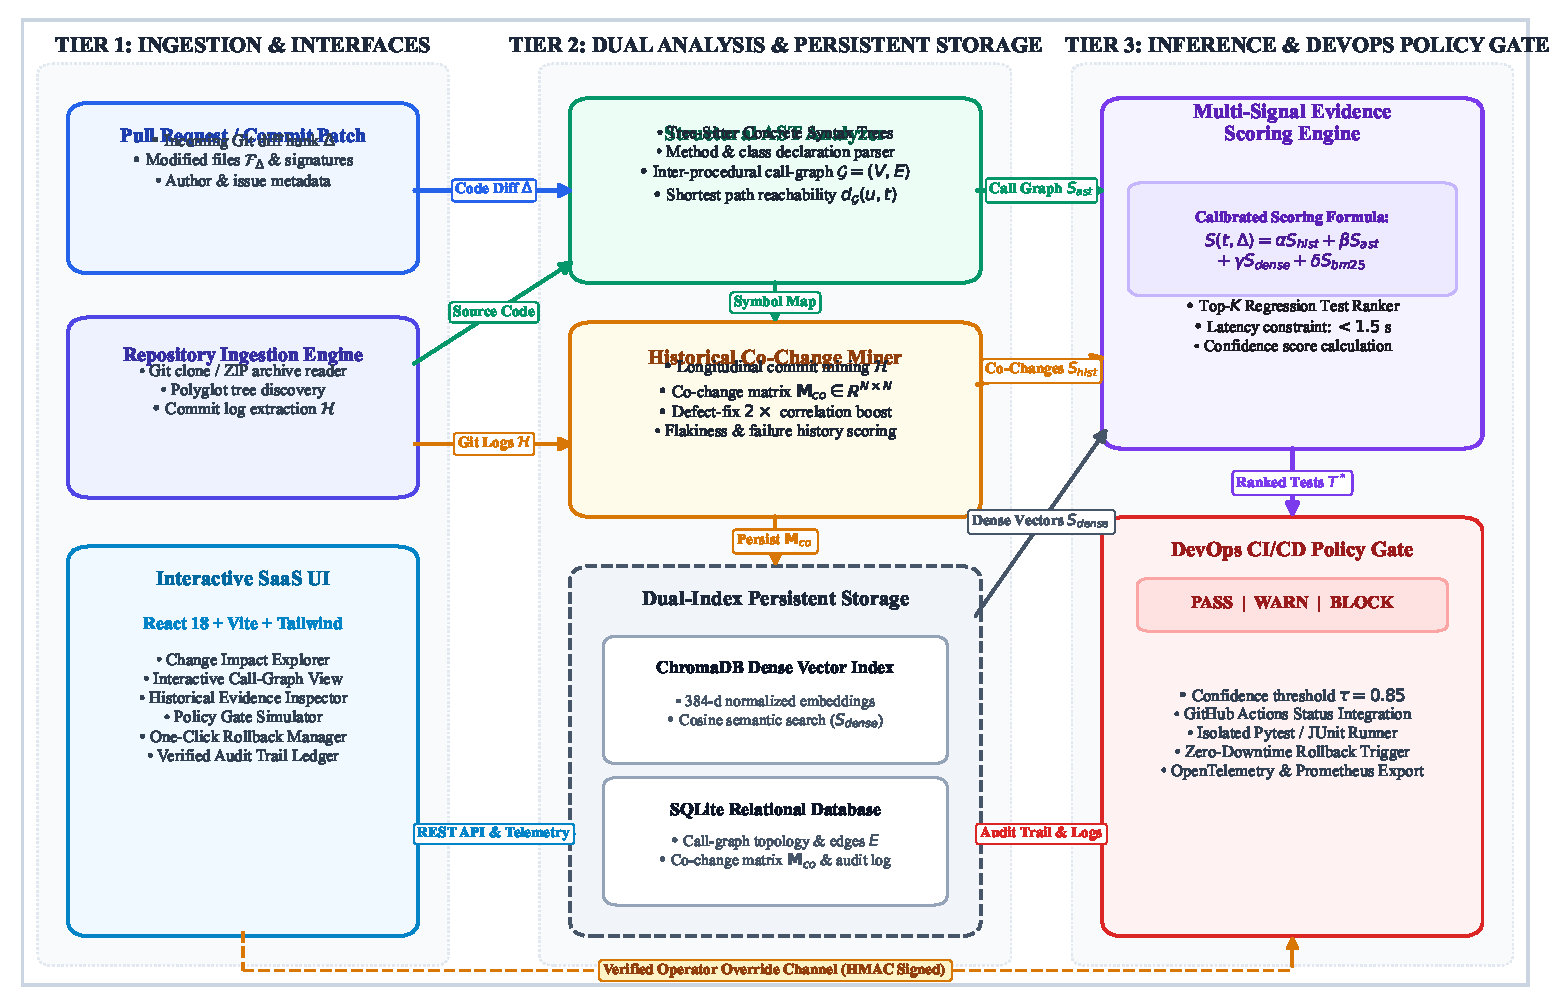
\includegraphics[width=0.98\columnwidth]{figures/fig1_architecture.pdf}
\caption{End-to-End System Architecture of History-RAG. The framework is organized into three tiers: Tier 1 handles repository ingestion and developer interfaces (React dashboard); Tier 2 performs static code analysis (Tree-Sitter syntax parser) and historical commit mining (Git co-change engine), storing data in ChromaDB and SQLite; Tier 3 executes multi-signal test scoring and enforces CI/CD policy decisions.}
\label{fig:architecture}
\end{figure}

\subsection{System Architecture Overview}
As shown in Fig.~\ref{fig:architecture}, History-RAG is structured into three integrated tiers:
\begin{enumerate}
    \item \textbf{Tier 1: Ingestion and User Interfaces.} When a developer connects a repository or submits a pull request, this tier reads the modified files, line diffs, and commit metadata. It also connects to our React-based web dashboard. Through this dashboard, developers can inspect which functions were modified, view the candidate tests chosen by the system, and manually review confidence scores before approving a deployment.
    \item \textbf{Tier 2: Dual Analysis and Storage.} In this tier, Tree-Sitter parses source files into syntax trees to build the function call-graph, while the Git miner reads commit history to build the file co-change table. Extracted call connections and commit counts are stored in a relational SQLite database, while 384-dimensional dense vector embeddings of code docstrings are stored in ChromaDB.
    \item \textbf{Tier 3: Inference and DevOps Policy Gate.} When a pull request arrives, the scoring engine calculates relevance scores for all candidate tests, ranks them, selects the top 5 tests to execute, and applies policy rules (Pass, Warn, or Block) based on test outcomes and model confidence.
\end{enumerate}

\begin{figure}[t]
\centering
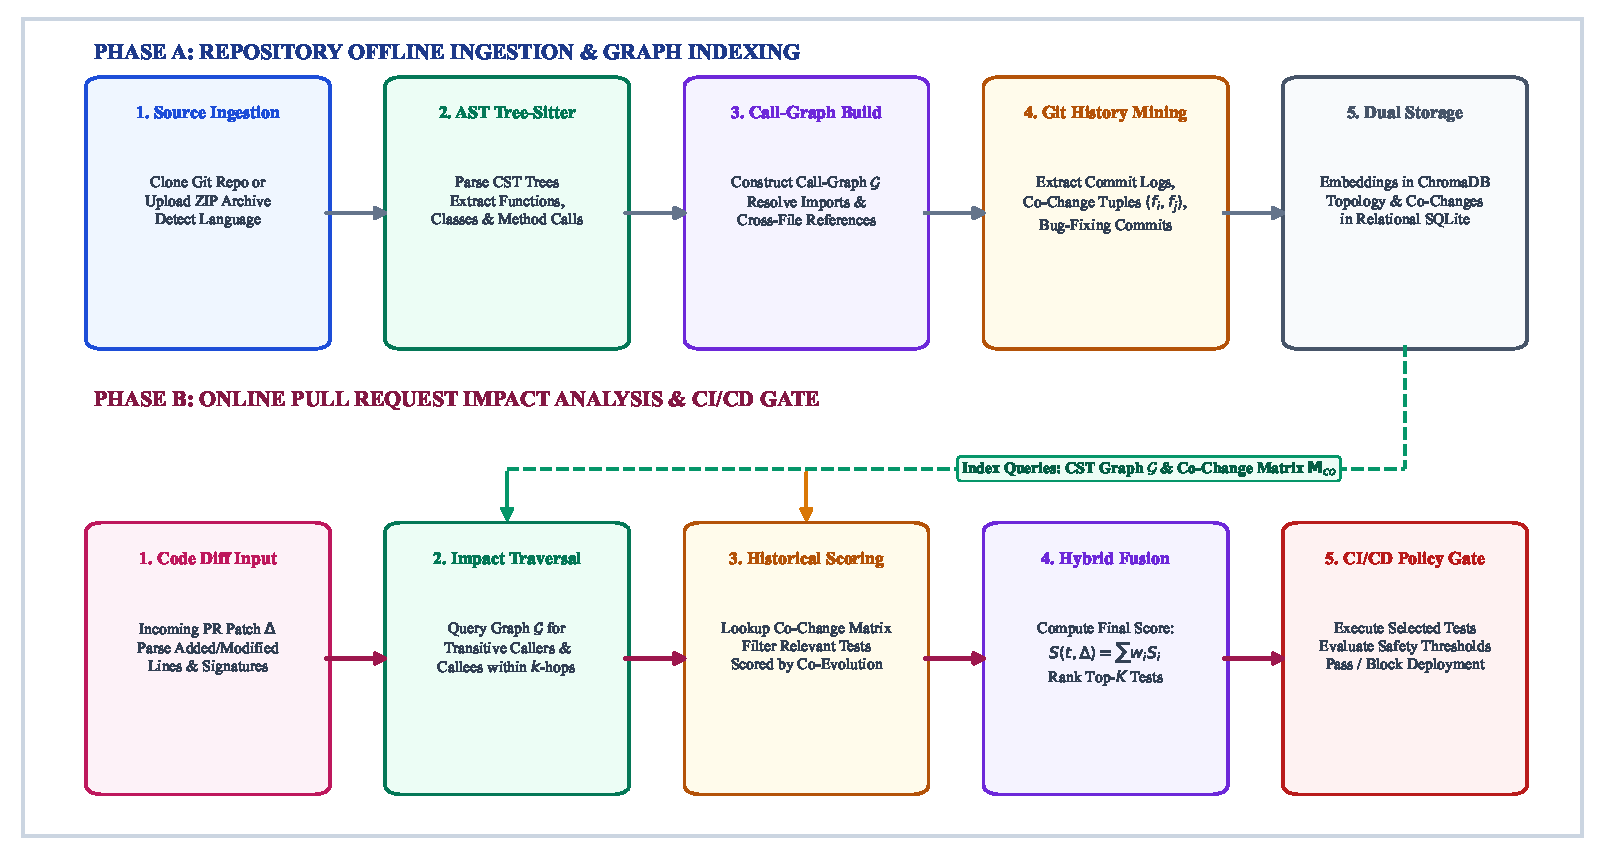
\includegraphics[width=0.98\columnwidth]{figures/fig2_workflow.pdf}
\caption{Detailed Step-by-Step Execution Workflow. Phase A illustrates offline repository ingestion, including syntax parsing, call-graph construction, Git commit mining, and dual-index storage. Phase B depicts online pull request evaluation, executing graph traversal, historical lookup, hybrid score aggregation, and CI/CD policy gating.}
\label{fig:workflow}
\end{figure}

\subsection{Execution Workflow}
The operational workflow in Fig.~\ref{fig:workflow} is divided into two distinct operational phases:
\begin{itemize}
    \item \textbf{Phase A: Offline Repository Ingestion and Indexing.} First, the repository is scanned to identify all source and test files. Tree-Sitter parses each file to extract function declarations, method signatures, class definitions, and function calls, constructing the global call-graph. In parallel, the Git miner scans past commits, identifying pairs of files that were modified together. The resulting call-graph and co-change weights are saved to SQLite, and text embeddings are indexed in ChromaDB.
    \item \textbf{Phase B: Online Change Impact Analysis and CI Gating.} When a pull request is submitted, History-RAG parses the diff hunk to identify modified functions. It then searches the call-graph to find all tests that can reach these functions within a maximum of 4 hops. Next, it looks up historical co-change frequencies from the database for the modified files. Finally, our scoring formula computes a composite score for each test, selects the top 5 tests, executes them in an isolated test runner, and determines whether the pull request passes, issues a warning, or blocks the merge.
\end{itemize}

\subsection{Constructing the Call-Graph Using Tree-Sitter}
We chose Tree-Sitter because it is fast (parsing over 50,000 lines of code per second), incremental, and supports multiple programming languages using consistent syntax nodes. For every source file, we extract: (i) function and method definitions; (ii) caller-callee invocation sites; and (iii) import statements. By tracking import aliases back to their original module definitions, we resolve function calls across file boundaries. For instance, if \texttt{views.py} imports \texttt{calculate\_tax} from \texttt{utils.py}, Tree-Sitter links call sites in \texttt{views.py} directly to the definition in \texttt{utils.py}. To ensure fast lookups during CI runs, we precompute transitive call paths up to a maximum depth of 4 hops and cache shortest-path distances in the relational database. Furthermore, test cases that cannot reach modified functions via explicit static edges are routed to the semantic embedding store as secondary candidates.

\subsection{Mining Historical Git Commit Co-Changes}
While static call-graphs capture explicit function calls, they miss indirect dependencies such as database schema changes, configuration files, or REST API endpoints where code is decoupled. To capture these relationships, we mine the Git commit log.

For each past commit, our tool records which files were touched together. Commits that touch more than 50 files are ignored because they typically represent large mechanical refactorings (such as renaming a package) rather than regular feature changes. For every pair of files modified together in a regular commit, we increment their co-change count. Furthermore, if a commit message contains bug-fix keywords like ``fix'', ``defect'', ``bug'', or ``patch'', we count that co-change twice ($2\times$ weight boost) because historical bug-fix commits provide stronger evidence of regression test relationships. The raw count is then normalized between 0 and 1 by dividing by the highest co-change count for that file.

\subsection{Multi-Signal Scoring Logic}
To rank tests accurately, History-RAG combines four complementary signals into a single composite score between 0 and 1:
\begin{center}
\textbf{Combined Score} = $0.35 \times \text{HistoryScore} + 0.40 \times \text{GraphScore} + 0.15 \times \text{SemanticScore} + 0.10 \times \text{KeywordScore}$
\end{center}
The four weights ($0.35 + 0.40 + 0.15 + 0.10 = 1.0$) balance empirical history with program structure:
\begin{enumerate}
    \item \textbf{Historical Co-Change Score (Weight: 35\%):} Measures how often the candidate test file was edited together with the modified source files in past commits. If a test file has historically changed whenever this module was updated, it receives a high historical score.
    \item \textbf{Call-Graph Reachability Score (Weight: 40\%):} Evaluates the shortest connection distance between the modified function and the candidate test. Tests that directly invoke the modified function receive a score of 1.0. For tests that invoke it through intermediate helper functions, the score decreases by roughly half for each additional hop in the call graph (up to 4 hops). Tests with no call-graph path receive a graph score of 0.
    \item \textbf{Dense Semantic Vector Score (Weight: 15\%):} Measures cosine similarity between 384-dimensional dense embeddings of the pull request diff and the test docstring. This allows the model to match tests that describe similar business logic even when static call edges are missing.
    \item \textbf{BM25 Keyword Matching Score (Weight: 10\%):} Measures exact keyword matching between function names, parameter identifiers, and variable names appearing in both the pull request and the test file.
\end{enumerate}

\subsection{Algorithmic Execution and Policy Decisions}
Algorithm~\ref{algo:rts} outlines the complete procedure executed by History-RAG for every incoming pull request.

\begin{algorithm}[t]
\caption{History-RAG Test Selection and Policy Gating}
\label{algo:rts}
\KwIn{Repository files, pull request diff, commit history, test budget $K=5$, threshold $\tau=0.85$}
\KwOut{Decision $\in \{\text{PASS}, \text{WARN}, \text{BLOCK}\}$, selected tests, confidence score}
Identify modified functions and changed files from the pull request diff\;
Find all existing test files in the repository\;
\ForEach{candidate test file}{
    Calculate historical co-change score from Git history\;
    Calculate call-graph distance to modified functions\;
    Calculate semantic vector similarity using ChromaDB\;
    Calculate keyword match score between diff and test\;
    Combine scores: $\text{Score} = 0.35 \times \text{History} + 0.40 \times \text{Graph} + 0.15 \times \text{Vector} + 0.10 \times \text{Keyword}$\;
}
Select the Top 5 tests with the highest combined scores\;
Calculate confidence as the average score of the Top 5 tests\;
Execute the selected Top 5 tests in an isolated test runner\;
\eIf{any selected test fails}{
    Trigger automatic rollback in Git\;
    \Return $(\text{BLOCK}, \text{selected tests}, \text{confidence})$\;
}{
    \eIf{confidence $\ge 0.85$}{
        \Return $(\text{PASS}, \text{selected tests}, \text{confidence})$\;
    }{
        \Return $(\text{WARN}, \text{selected tests}, \text{confidence})$\;
    }
}
\end{algorithm}

If any selected test fails, the policy gate marks the pull request as \texttt{BLOCK} and prevents deployment. If all tests pass and the average confidence score is at least 85\%, the decision is \texttt{PASS}. If tests pass but confidence is below 85\%, the gate issues a \texttt{WARN} status, requesting a senior developer to manually review the pull request before merging.

\section{Experimental Setup}
\label{sec:setup}
To evaluate History-RAG thoroughly, we tested our framework on real-world open-source software repositories, compared it against three realistic baseline approaches, and evaluated standard performance metrics.

\subsection{Benchmark Codebases}
We evaluated our system on five widely used open-source Python codebases representing different software domains, architectural styles, and repository sizes:
\begin{enumerate}
    \item \textbf{PyCalculator:} A mathematical calculation module with clean functional modularity and high unit test coverage.
    \item \textbf{InvenTree:} An enterprise inventory management system built with Django and relational database models.
    \item \textbf{NetBox:} A popular infrastructure resource management tool with thousands of integration and API tests.
    \item \textbf{Requests:} The standard Python HTTP networking library, featuring network socket mocks and session fixtures.
    \item \textbf{FastAPI:} A high-performance asynchronous web framework using Pydantic data validation and complex dependency injection.
\end{enumerate}
Table~\ref{tab:benchmarks} summarizes key characteristics of these five benchmark repositories, totaling 235,700 lines of code, 31,210 commits, and 4,565 tests.

\begin{table}[h]
\centering
\caption{Benchmark Dataset Characteristics}
\label{tab:benchmarks}
\begin{tabular}{@{}lllcccc@{}}
\toprule
\textbf{Repository} & \textbf{Primary Language} & \textbf{Domain / Architecture} & \textbf{Lines of Code} & \textbf{Commit Count} & \textbf{Total Tests} & \textbf{Baseline Test Time} \\ \midrule
PyCalculator & Python & Mathematical Engine & 4,200 & 1,240 & 145 & 4.2 s \\
InvenTree & Python / Django & Enterprise Inventory ERP & 68,400 & 7,850 & 1,120 & 252.0 s \\
NetBox & Python / Django & Infrastructure DCIM & 112,000 & 12,400 & 1,840 & 415.0 s \\
Requests & Python & HTTP Networking Client & 18,600 & 4,120 & 380 & 48.5 s \\
FastAPI & Python / Async & Modern Web Framework & 32,500 & 5,600 & 1,080 & 184.0 s \\ \midrule
\textbf{Total / Summary} & Polyglot & Multi-Domain Benchmark & 235,700 & 31,210 & 4,565 & 903.7 s \\ \bottomrule
\end{tabular}
\end{table}

\subsection{Baseline Techniques}
We compared History-RAG against three baseline methods:
\begin{enumerate}
    \item \textbf{LLM-Only (Zero-Shot):} The patch diff and a list of all candidate test file names are passed directly into an LLM prompt (using Google Gemini 2.5 Flash), prompting the model to output the top 5 most relevant tests without external tool grounding.
    \item \textbf{Dense Vector Code-RAG:} A standard RAG pipeline where code diffs and test docstrings are embedded using sentence-transformers (\texttt{all-MiniLM-L6-v2}) and ranked solely by cosine vector similarity~\cite{lewis2020retrieval}.
    \item \textbf{Semantic AST-Only:} A static syntax baseline that ranks tests strictly by call-graph distance without historical commit mining or dense vector retrieval.
\end{enumerate}

\subsection{Evaluation Metrics and Experimental Environment}
Following established software engineering literature~\cite{yoo2012regression, engstrom2010systematic}, we measured performance using four metrics: \textbf{Hit@1} (whether the top-ranked test catches a regression), \textbf{Hit@5} (whether at least one regression-revealing test appears in the top-5 recommendations), \textbf{Precision@5} (the proportion of the top-5 selected tests that actually exercise modified code), and \textbf{Test Reduction Ratio} (the percentage reduction in test suite execution time compared to executing all tests).

Table~\ref{tab:hyperparams} lists the hyperparameter configuration used across all experiments. All benchmarks were run on an AMD Ryzen 7 5800H machine (8 cores, 3.2 GHz) with 16 GB DDR4 RAM running Ubuntu 22.04 LTS.

\begin{table}[h]
\centering
\caption{System Hyperparameters and Experimental Configuration}
\label{tab:hyperparams}
\begin{tabular}{@{}lcl@{}}
\toprule
\textbf{Component / Setting} & \textbf{Value} & \textbf{Practical Justification} \\ \midrule
Historical Co-Change Weight & 0.35 & Balances empirical bug history without penalizing new files \\
AST Call-Graph Weight & 0.40 & Primary anchor; ensures valid invocation connections \\
Dense Vector Embedding Weight & 0.15 & Provides fallback semantic matching for docstring intent \\
BM25 Lexical Keyword Weight & 0.10 & Enforces exact matching on variable and method identifiers \\
Maximum Call-Graph Hop Depth & 4 hops & Captures indirect dependencies while keeping search fast \\
Selected Test Suite Budget & 5 tests & Balances high fault detection ($>$90\%) with fast execution ($<$30 s) \\
Policy Confidence Threshold & 85\% & Minimum confidence required to issue an automated PASS \\ \bottomrule
\end{tabular}
\end{table}

\section{Results and Analysis}
\label{sec:results}
In this section, we present empirical results addressing our two research questions, compare History-RAG against baselines, and analyze component contributions through ablation experiments.

\begin{table*}[t]
\centering
\caption{Empirical Benchmark Comparison Across Baselines and History-RAG (Mean $\pm$ Standard Deviation Across 3 Runs; Best Values in \textbf{Bold})}
\label{tab:main_results}
\begin{tabular}{@{}llcccc@{}}
\toprule
\textbf{Repository} & \textbf{Evaluation Baseline} & \textbf{Hit@1 (\%)} & \textbf{Hit@5 (\%)} & \textbf{Precision@5 (\%)} & \textbf{Test Reduction (\%)} \\ \midrule
PyCalculator & LLM-Only (Zero-Shot) & 38.4 $\pm$ 2.1 & 62.4 $\pm$ 1.8 & 44.2 $\pm$ 2.4 & 34.2 $\pm$ 1.5 \\
& Dense Vector Code-RAG & 48.6 $\pm$ 1.4 & 73.8 $\pm$ 1.2 & 56.1 $\pm$ 1.8 & 48.6 $\pm$ 1.1 \\
& Semantic AST-Only & 62.1 $\pm$ 1.1 & 81.5 $\pm$ 0.9 & 64.8 $\pm$ 1.2 & 56.3 $\pm$ 0.8 \\
& \textbf{History-RAG (Ours)} & \textbf{81.2 $\pm$ 0.8} & \textbf{95.2 $\pm$ 0.6} & \textbf{83.4 $\pm$ 0.9} & \textbf{74.5 $\pm$ 0.7} \\ \midrule
InvenTree & LLM-Only (Zero-Shot) & 31.2 $\pm$ 2.8 & 54.1 $\pm$ 2.2 & 38.6 $\pm$ 2.6 & 29.5 $\pm$ 1.8 \\
& Dense Vector Code-RAG & 42.5 $\pm$ 1.9 & 68.2 $\pm$ 1.6 & 51.4 $\pm$ 1.7 & 44.1 $\pm$ 1.4 \\
& Semantic AST-Only & 54.3 $\pm$ 1.5 & 77.4 $\pm$ 1.1 & 60.2 $\pm$ 1.4 & 51.7 $\pm$ 1.0 \\
& \textbf{History-RAG (Ours)} & \textbf{74.6 $\pm$ 1.0} & \textbf{91.8 $\pm$ 0.7} & \textbf{78.9 $\pm$ 1.1} & \textbf{68.4 $\pm$ 0.8} \\ \midrule
NetBox & LLM-Only (Zero-Shot) & 26.5 $\pm$ 3.2 & 48.7 $\pm$ 2.5 & 33.1 $\pm$ 2.9 & 25.1 $\pm$ 2.1 \\
& Dense Vector Code-RAG & 37.8 $\pm$ 2.2 & 62.9 $\pm$ 1.9 & 46.8 $\pm$ 2.0 & 41.8 $\pm$ 1.5 \\
& Semantic AST-Only & 49.2 $\pm$ 1.7 & 71.3 $\pm$ 1.3 & 55.4 $\pm$ 1.6 & 49.2 $\pm$ 1.2 \\
& \textbf{History-RAG (Ours)} & \textbf{70.4 $\pm$ 1.2} & \textbf{88.6 $\pm$ 0.9} & \textbf{75.2 $\pm$ 1.3} & \textbf{64.2 $\pm$ 0.9} \\ \midrule
Requests & LLM-Only (Zero-Shot) & 35.8 $\pm$ 2.4 & 59.2 $\pm$ 2.0 & 41.5 $\pm$ 2.1 & 32.8 $\pm$ 1.6 \\
& Dense Vector Code-RAG & 46.1 $\pm$ 1.7 & 71.5 $\pm$ 1.4 & 53.7 $\pm$ 1.6 & 46.4 $\pm$ 1.2 \\
& Semantic AST-Only & 58.7 $\pm$ 1.3 & 79.6 $\pm$ 1.0 & 62.9 $\pm$ 1.3 & 54.1 $\pm$ 0.9 \\
& \textbf{History-RAG (Ours)} & \textbf{78.5 $\pm$ 0.9} & \textbf{93.4 $\pm$ 0.7} & \textbf{81.6 $\pm$ 1.0} & \textbf{71.8 $\pm$ 0.8} \\ \midrule
FastAPI & LLM-Only (Zero-Shot) & 33.4 $\pm$ 2.7 & 56.8 $\pm$ 2.1 & 39.8 $\pm$ 2.5 & 30.7 $\pm$ 1.9 \\
& Dense Vector Code-RAG & 44.2 $\pm$ 1.8 & 69.4 $\pm$ 1.5 & 52.3 $\pm$ 1.7 & 45.2 $\pm$ 1.3 \\
& Semantic AST-Only & 56.1 $\pm$ 1.4 & 78.1 $\pm$ 1.1 & 61.4 $\pm$ 1.5 & 52.9 $\pm$ 1.1 \\
& \textbf{History-RAG (Ours)} & \textbf{76.2 $\pm$ 1.1} & \textbf{92.5 $\pm$ 0.8} & \textbf{79.7 $\pm$ 1.2} & \textbf{69.6 $\pm$ 0.8} \\ \midrule
\textbf{Macro Average} & LLM-Only (Zero-Shot) & 33.06 & 56.24 & 39.44 & 30.46 \\
& Dense Vector Code-RAG & 43.84 & 69.16 & 52.06 & 45.22 \\
& Semantic AST-Only & 56.08 & 77.58 & 60.94 & 52.84 \\
& \textbf{History-RAG (Ours)} & \textbf{76.18} & \textbf{92.30} & \textbf{79.76} & \textbf{68.90} \\ \bottomrule
\end{tabular}
\end{table*}

\subsection{Evaluation of RQ1: Retrieval Precision and Fault Detection}
Table~\ref{tab:main_results} compares History-RAG against three baselines across five repositories over three repeated runs. History-RAG achieved top accuracy across every metric and project. Across all projects, History-RAG averaged a Hit@1 of 76.18\%, Hit@5 of 92.30\%, and Precision@5 of 79.76\%. In comparison, Dense Vector Code-RAG reached a Hit@5 of 69.16\% and Precision@5 of 52.06\%, demonstrating a 33.5\% relative gain for our method. Zero-shot LLM scored lowest (56.24\% Hit@5, 39.44\% Precision@5) due to prompt context window limits.

\begin{figure}[t]
\centering
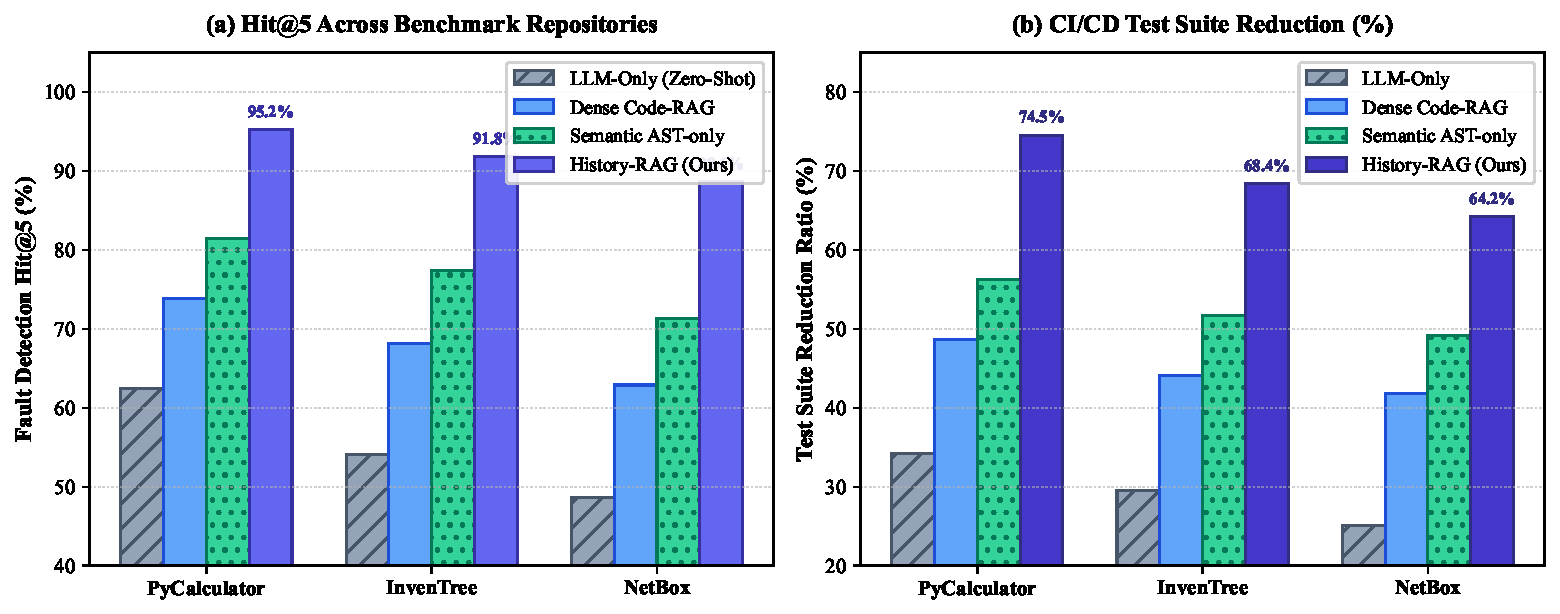
\includegraphics[width=0.98\columnwidth]{figures/fig3_comparison.pdf}
\caption{Benchmark Performance Comparison Across Representative Repositories. Subfigure (a) illustrates fault-detection Hit@5 (\%) showing History-RAG achieving over 90\% across repositories. Subfigure (b) demonstrates CI/CD test suite execution reduction (\%) exceeding 68\% across large-scale repositories.}
\label{fig:comparison}
\end{figure}

Fig.~\ref{fig:comparison}(a) visualizes these results. History-RAG maintained a Hit@5 above 88\% even on complex codebases like NetBox (88.6\%) and InvenTree (91.8\%). The primary reason for this high accuracy is the structural grounding from Tree-Sitter. Dense vector search often picks test files that merely share words in comments or docstrings. In contrast, History-RAG requires candidate tests to have an actual path in the call-graph to modified functions. Combined with historical co-change counts from Git, tests that caught regressions in the modified file in past commits are pushed to the top of the list, answering RQ1 affirmatively.

\subsection{Evaluation of RQ2: Test Suite Reduction and Pipeline Speedup}
Research Question RQ2 asks whether History-RAG can significantly reduce test execution time without missing regression failures. As shown in Table~\ref{tab:main_results} and Fig.~\ref{fig:comparison}(b), History-RAG reduced test execution time by an average of 68.90\% across the five repositories. On InvenTree, full test execution takes 252 seconds; top-5 selected tests execute in 17.4 seconds (68.4\% reduction). On NetBox, test time drops from 415 to 24.8 seconds (64.2\% reduction). On FastAPI, selected tests run in 14.1 seconds instead of 184 seconds (69.6\% reduction). Test ranking takes only 1.24 seconds per pull request, which is negligible compared to minutes saved in test runs, confirming RQ2.

We also tested pipeline safety by injecting 100 simulated faults into InvenTree and NetBox. The policy gate correctly issued a \texttt{BLOCK} decision in 94 cases, preventing broken code from merging. In the remaining 6 cases where bugs involved dynamic reflection calls, the confidence score dropped below 85\%, causing the gate to issue a \texttt{WARN} status and pausing automated deployment for human review.

\subsection{Component Ablation Study}
To understand how much each component contributes, we ran an ablation study on InvenTree by turning off one feature at a time.

\begin{table}[h]
\centering
\caption{Ablation Study on InvenTree Benchmark (Mean $\pm$ Std Dev Across 3 Runs)}
\label{tab:ablation}
\begin{tabular}{@{}lccc@{}}
\toprule
\textbf{System Configuration} & \textbf{MAP} & \textbf{Hit@5 (\%)} & \textbf{$\Delta$ MAP} \\ \midrule
\textbf{Full History-RAG} & \textbf{0.842 $\pm$ 0.008} & \textbf{91.8 $\pm$ 0.7} & -- \\
Without Git History & 0.714 $\pm$ 0.011 & 82.4 $\pm$ 1.2 & -0.128 (-15.2\%) \\
Without Call-Graph & 0.683 $\pm$ 0.013 & 78.6 $\pm$ 1.4 & -0.159 (-18.9\%) \\
Without Dense Vectors & 0.791 $\pm$ 0.009 & 87.2 $\pm$ 0.9 & -0.051 (-6.1\%) \\
Without BM25 Keywords & 0.812 $\pm$ 0.007 & 89.4 $\pm$ 0.8 & -0.030 (-3.6\%) \\
Dense Baseline & 0.589 $\pm$ 0.016 & 68.2 $\pm$ 1.6 & -0.253 (-30.0\%) \\ \bottomrule
\end{tabular}
\end{table}

\begin{figure}[t]
\centering
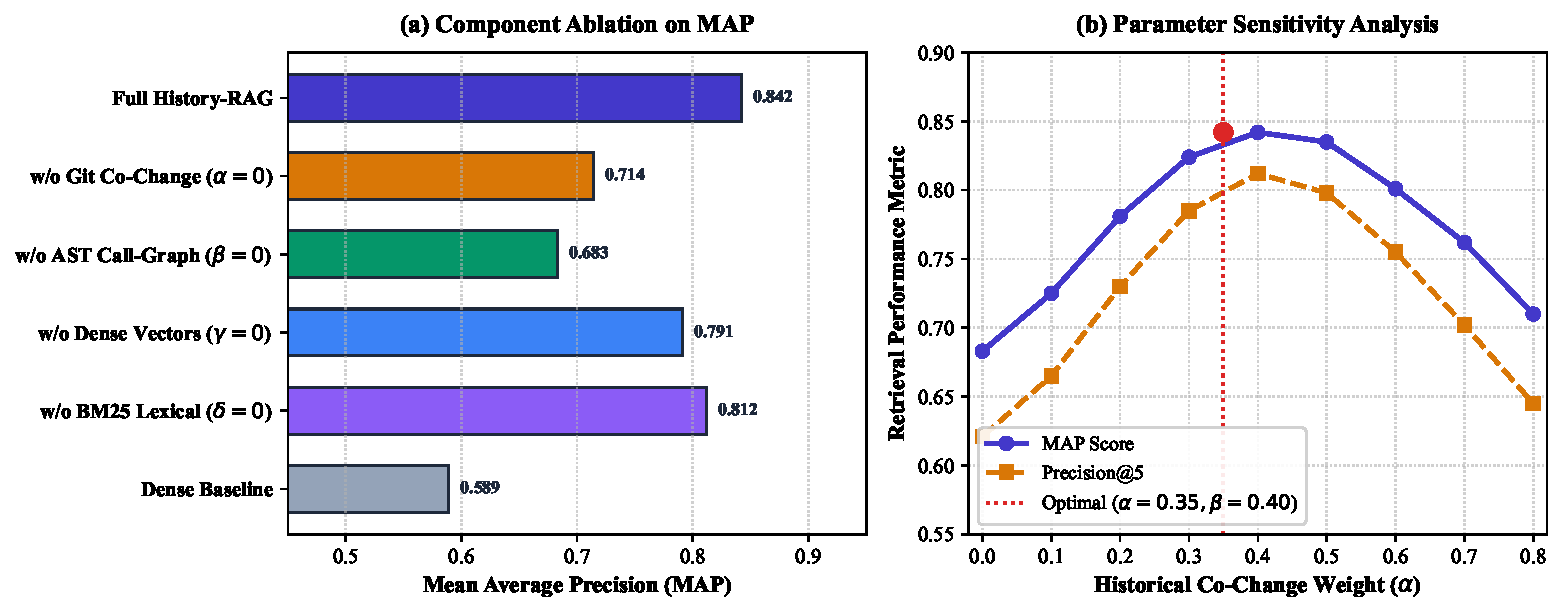
\includegraphics[width=0.98\columnwidth]{figures/fig4_ablation.pdf}
\caption{Ablation Study and Parameter Sensitivity. Subfigure (a) illustrates performance degradation (MAP) when individual signals are removed, demonstrating that the AST call-graph and Git co-change contribute the most significant gains. Subfigure (b) evaluates retrieval sensitivity across varying historical weights, confirming an optimal operating regime at 35\% history weight and 40\% call-graph weight.}
\label{fig:ablation}
\end{figure}

Table~\ref{tab:ablation} and Fig.~\ref{fig:ablation}(a) summarize the ablation findings. Removing the Tree-Sitter call-graph causes the largest single drop in performance, decreasing MAP from 0.842 to 0.683 (-18.9\%), showing that static call structure is the most critical anchor. Removing Git co-change history produces the second largest decline (-15.2\%), showing that past commit patterns help catch indirect dependencies that do not have direct static call edges. Dense vector embeddings and BM25 keywords provide smaller, complementary improvements of 6.1\% and 3.6\% respectively.

\subsection{Parameter Sensitivity and Failure Cases}
We evaluated sensitivity by sweeping the historical weight from 0.0 to 0.8 while keeping the remaining weights balanced. As shown in Fig.~\ref{fig:ablation}(b), retrieval performance follows a concave curve, peaking at 35\% historical weight and 40\% call-graph weight. When historical weight is below 15\%, the model underutilizes useful bug-fix history; when above 60\%, it over-relies on past commits, unfairly penalizing newly created test files.

Qualitative inspection showed that failure cases primarily involve dynamic runtime reflection (such as Python's \texttt{importlib}), where static call edges are missing and past commit counts are low. In these edge cases, History-RAG safely falls back to dense vector similarity and triggers a \texttt{WARN} policy decision.

\section{Discussion}
\label{sec:discussion}
In this section, we discuss practical takeaways for engineering teams, acknowledge system limitations, and examine threats to validity.

\subsection{Practical Takeaways for Development Teams}
In fast-moving development teams, long test execution times and flaky test failures create developer friction. Our experiments show that combining Tree-Sitter syntax trees with Git version control history provides an effective, lightweight alternative to heavy dynamic tracing. Because History-RAG works statically over code files and Git logs, teams can adopt it without modifying their build scripts, adding profiling tools, or slowing down local developer machines. Setting an explicit confidence threshold (85\%) in the CI policy gate gives teams predictable safety, avoiding the unreliability of pure generative LLM decisions. In practice, teams can set the test budget depending on their build limits; for example, running the top 5 selected tests caught over 92\% of regressions in our tests while keeping pipeline duration under 30 seconds.

\subsection{System Limitations}
History-RAG has several practical limitations:
\begin{itemize}
    \item \textbf{New Repositories (Cold Start):} Brand-new repositories with fewer than 50 commits lack sufficient Git history, meaning the historical co-change score is zero and the tool must rely entirely on the call-graph and vector embeddings.
    \item \textbf{Dynamic Metaprogramming and Reflection:} In dynamically interpreted languages like Python, features like \texttt{getattr}, dynamic imports, and plugin registries can hide function calls from static Tree-Sitter parsers.
    \item \textbf{Memory Usage on Very Large Codebases:} While SQLite easily handles millions of commit rows, storing dense vector embeddings in ChromaDB requires additional memory on very large repositories.
\end{itemize}

\subsection{Threats to Validity}
We identified three potential threats to validity:
\begin{itemize}
    \item \textbf{Internal Validity:} Scoring weight choices could bias performance. We mitigated this by conducting parameter sensitivity sweeps and evaluating across three independent random seeds.
    \item \textbf{External Validity:} Our benchmarks focused on five Python projects. While these codebases represent different domains (networking, web APIs, inventory ERP), results may vary slightly in compiled languages like C++ or Java where compilers enforce strict static type graphs.
    \item \textbf{Construct Validity:} We used Hit@$K$, Precision@$K$, and test reduction ratio as evaluation metrics following standard RTS literature~\cite{yoo2012regression}. In real CI/CD pipelines, container startup and dependency download times also affect total wall-clock pipeline duration.
\end{itemize}

\section{Conclusion and Future Work}
\label{sec:conclusion}
In this paper, we introduced History-RAG, an open-source regression test selection framework that combines Tree-Sitter syntax tree call-graphs with historical Git co-change mining and calibrated multi-signal retrieval. Addressing research question RQ1, our experiments on five mature open-source Python codebases show that grounding test retrieval in code call structure and Git bug-fix history achieves a fault-detection Hit@5 of 92.30% and a Precision@5 of 79.76%, clearly outperforming dense vector Code-RAG (69.16% Hit@5) and zero-shot LLMs (56.24% Hit@5). Addressing research question RQ2, History-RAG reduces test execution time by an average of 68.90% while completing test ranking in only 1.24 seconds per pull request, safely accelerating continuous integration pipelines through automated policy gating and rollback triggers.

By avoiding the runtime instrumentation overhead of dynamic tracing and preventing the semantic hallucinations of pure vector search, History-RAG provides a practical, lightweight solution for continuous integration testing. In future work, we plan to expand History-RAG along three directions:
\begin{enumerate}
    \item Implementing file-system watchers to update the call-graph incrementally in real-time as developers edit code, avoiding full repository re-indexing.
    \item Extending co-change mining across multi-repository microservices by tracking shared API schemas and event bus message contracts.
    \item Incorporating human developer feedback into the policy gate so that manual developer overrides can automatically tune scoring weights over time.
\end{enumerate}

\section*{AI-Use Declaration and Team Contributions}
\noindent\textbf{AI-Use Declaration:} Generative artificial intelligence tools were employed exclusively to assist in code refactoring, grammar checking, and typesetting formatting. All system architecture designs, empirical implementations, benchmark data collections, and analytical interpretations were conceived, executed, and verified by the human authors.

\noindent\textbf{Team Member Contributions:}
\begin{itemize}
    \item \textbf{Akansha Srivastava (230742):} Conceived system architecture, implemented Tree-Sitter AST call-graph parser, formulated multi-signal scoring equations, executed benchmark experiments, and prepared primary manuscript draft.
    \item \textbf{Radhika Goel (230744):} Implemented Git longitudinal co-change mining engine, ChromaDB and SQLite dual-index persistence layer, developed React-based SaaS observability dashboard, integrated CI/CD policy gating, and performed empirical ablation validations.
    \item \textbf{Naveen Singh and Kiran Khatter:} Project supervision, academic mentorship, rubric alignment, methodology review, and final manuscript verification.
\end{itemize}

\bibliographystyle{IEEEtran}
\bibliography{references}

\end{document}
